% Name: Permutation and its cycles
% Description: A permutation of 1 to 7 in two-line notation and drawn as arrows, falling apart into the cycles (1 3 5), (2 7), (4), and (6).
% Tags: permutation, cycle notation, symmetric group, combinatorics

\usepackage{amsmath}
\usetikzlibrary{arrows.meta}

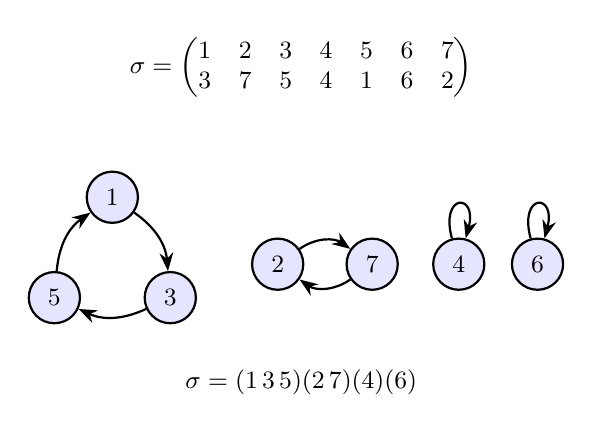
\begin{tikzpicture}[>={Stealth}, thick, every node/.style={font=\small},
    v/.style={circle, draw, fill=blue!10, minimum size=6.5mm, inner sep=0pt}]
  \node at (-1.2,0.9) {$\sigma = \begin{pmatrix} 1 & 2 & 3 & 4 & 5 & 6 & 7 \\ 3 & 7 & 5 & 4 & 1 & 6 & 2 \end{pmatrix}$};
  % Each cycle on its own: 1 → 3 → 5 → 1, 2 → 7 → 2, and the fixed points 4 and 6
  \begin{scope}[shift={(-3.6,-1.6)}]
    \foreach \v/\a in {1/90, 3/-30, 5/210} \node[v] (c\v) at (\a:0.85) {\v};
    \draw[->] (c1) to[bend left=25] (c3);
    \draw[->] (c3) to[bend left=25] (c5);
    \draw[->] (c5) to[bend left=25] (c1);
  \end{scope}
  \node[v] (c2) at (-1.5,-1.6) {2};
  \node[v] (c7) at (-0.3,-1.6) {7};
  \draw[->] (c2) to[bend left=35] (c7);
  \draw[->] (c7) to[bend left=35] (c2);
  \foreach \v/\x in {4/0.8, 6/1.8} {
    \node[v] (c\v) at (\x,-1.6) {\v};
    \draw[->] (c\v) edge[loop above, min distance=6mm] (c\v);
  }
  \node at (-1.2,-3.1) {$\sigma = (1\,3\,5)(2\,7)(4)(6)$};
\end{tikzpicture}
